\section{Uneigentliche Integrale}\label{sec:uneigentliche-integrale}

Ein \textbf{uneigentliches Integral} hat die Eigenschaft, dass der Integrationsbereich unendlich gross ist oder eine Polstelle enthält.

\subsection{Uneigentlicher Integrationsbereich}\label{subsec:uneigentlicher-integrationsbereich}

\begin{definition}{Definition}
    \begin{multicols}{2}
        \[\int_{a}^{\infty} f(x) \diff{x} = \lim_{t \rightarrow \infty} \int_{a}^{t} f(x) \diff{x}\] Dieses ``uneigentliche Integral'' existiert also, wenn der Grenzwert auf der rechten Seite der obigen Gleichung existiert.

        \begin{center}
            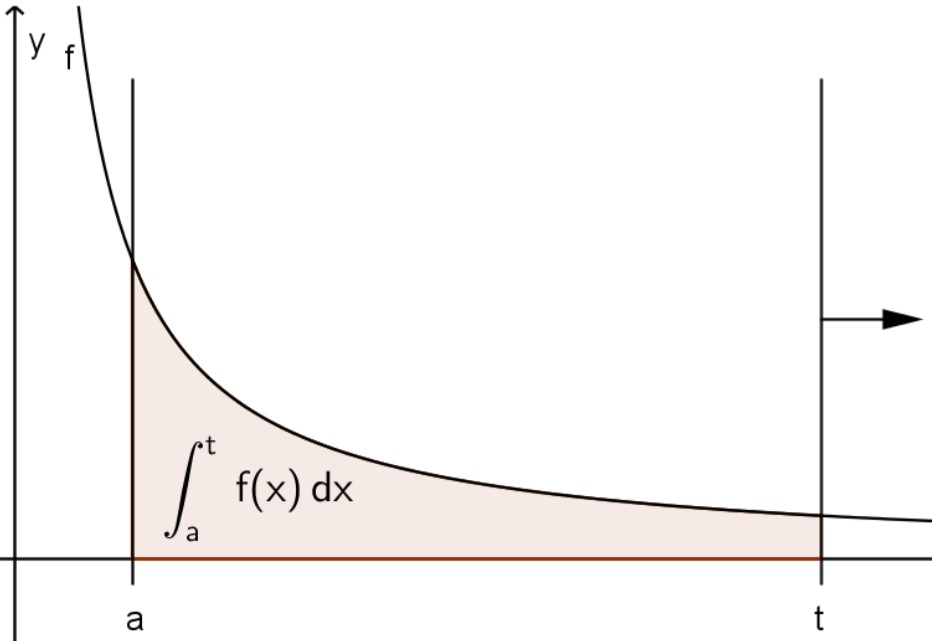
\includegraphics[scale=0.2]{uneigentlicher-integral}
        \end{center}
    \end{multicols}
\end{definition}

\textbf{Bemerkung:} Für die untere Grenze gilt entsprechend: $\int \limits_{-\infty}^{b} f(x) \diff{x} = \lim \limits_{t \rightarrow -\infty} \int \limits_{t}^{b} f(x) \diff{x}$

\textbf{Beispiele:}
\begin{multicols}{2}
    \begin{itemize}
        \item $\int \limits_{1}^{\infty} \frac{1}{x^2} \diff{x} \Rightarrow \int \limits_{1}^{t} \frac{1}{x^2} \diff{x} = \left[ -\frac{1}{x} \right]_{1}^{t} = -\frac{1}{t} + 1 \xrightarrow[t \to \infty]{} 1$
        \item $\int \limits_{-\infty}^{0} e^x \diff{x} \Rightarrow \int \limits_{t}^{0} e^x \diff{x} = \left[ e^x \right]_{t}^{0} = 1 - e^t \xrightarrow[t \to -\infty]{} 1$
        \item $\int \limits_{1}^{\infty} \frac{1}{x} \diff{x} \Rightarrow \int \limits_{1}^{t} \frac{1}{x} \diff{x} = \left[ \ln(|x|) \right]_{1}^{t} = \ln(t) - \ln(1) \xrightarrow[t \to \infty]{} \infty$ \\
        (Das Integral existiert also nicht)
    \end{itemize}
\end{multicols}

\subsection{Integrale über Polstellen der Funktion}\label{subsec:integrale-uber-polstellen-der-funktion}

\begin{definition}{Definition}
    \begin{multicols}{2}
        Gegeben ist eine Funktion $f$, die auf einem Intervall $(a, b]$ definiert und stetig ist, aber für $x \rightarrow a$ gegen unendlich strebt.
        Dann definieren wir: \[\int_{a}^{b} f(x) \diff{x} = \lim_{t \rightarrow a} \int_{t}^{a} f(x) \diff{x}\]
        Dieses ``uneigentliche Integral'' existiert also, wenn der entsprechende Grenzwert auf der rechten Seite der obigen Gleichung existiert.

        \begin{center}
            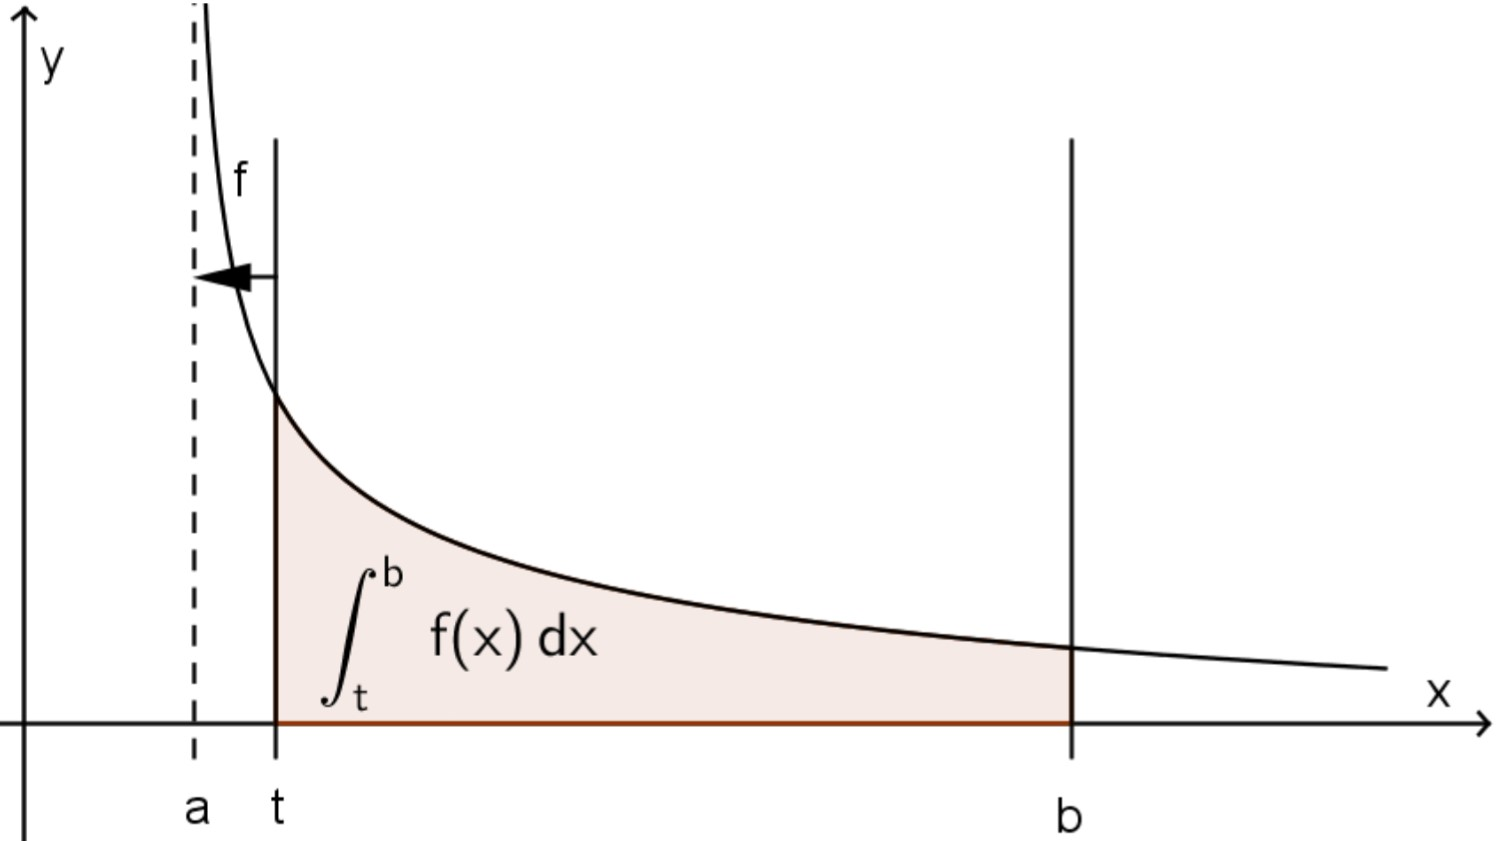
\includegraphics[scale=0.18]{uneigentlicher-integral-2}
        \end{center}
    \end{multicols}
\end{definition}

\textbf{Bemerkung:} Falls die Funktion auf der rechten Seite gegen unendlich strebt, dann lässt sich die obige Definition entsprechend anpassen:
\[\int \limits_{a}^{b} f(x) \diff{x} = \lim_{t \to b} \int \limits_{a}^{t} f(x) \diff{x}\]

\textbf{Beispiele:}
\begin{itemize}
    \item $\displaystyle \int \limits_{0}^{1} \frac{1}{\sqrt{x}} \diff{x} = \lim_{t \to 0} \int \limits_{t}^{1} \frac{1}{\sqrt {x}} \diff{x} = \lim_{t \to 0} \int \limits_{t}^{1} x^{-0.5} \diff{x} = \lim_{t \to 0} \left[ 2x^{0.5} \right]_{t}^{1} = 2 \sqrt{1} - 2 \sqrt {t} \xrightarrow[t \to 0]{} 2$
    \item $\displaystyle \int \limits_{0}^{1} \frac{1}{x} \diff{x} = \lim_{t \to 0} \int \limits_{t}^{1} \frac{1}{x} \diff{x} = \lim_{t \to 0} \left[ \ln(|x|) \right]_{t}^{1} = \lim_{t \to 0} \ln(1) - \ln(t) \xrightarrow[t \to 0]{} 0 - (-\infty) = \infty$ \\
    (Das Integral existiert also nicht)
\end{itemize}